\begin{question}
\noindent Triangle $T$ is drawn on the grid below.

\begin{center}
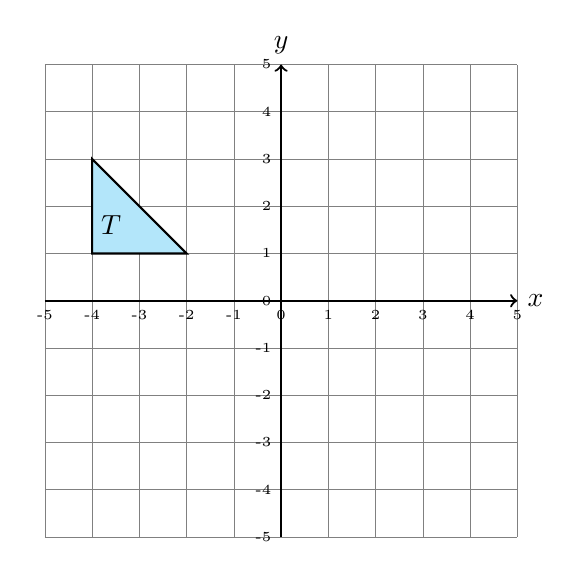
\begin{tikzpicture}[scale=0.6]
    \draw[step=1cm, gray, very thin] (-5,-5) grid (5,5);
    \draw[thick,->] (-5,0) -- (5,0) node[right] {$x$};
    \draw[thick,->] (0,-5) -- (0,5) node[above] {$y$};

    \foreach \x in {-5,-4,...,5}
        \node[below] at (\x,0) {\tiny \x};
    \foreach \y in {-5,-4,...,5}
        \node[left] at (0,\y) {\tiny \y};

    \draw[thick, fill=cyan!30] (-4,1) -- (-2,1) -- (-4,3) -- cycle;
    \node at (-3.6,1.6) {$T$};

\end{tikzpicture}
\end{center}

\noindent Translate triangle $T$ by the vector $\begin{pmatrix} 5 \\ -3 \end{pmatrix}$.

\noindent Draw the image of triangle $T$ on the grid and label it $T'$.

\vspace{4cm}

\begin{flushright}
\answermarks{2}
\end{flushright}
\end{question}